\section{Test Svolti}
In questa sezione si elencano i vari test che sono stati svolti, i problemi riscontrati e le soluzioni trovate.

\subsection{Controllo}
La prima fase sperimentale è stata dedicata alla verifica funzionale dei driver e del nodo ROS forniti da AgileX per il rover modello Hunter. L'obiettivo primario era determinare se tali componenti, specificamente progettati per il controllo e l'analisi del veicolo, potessero essere integrati nel sistema senza richiedere modifiche sostanziali o se, al contrario, fosse necessario apportare adattamenti o addirittura una completa riscrittura.

\noindent Per condurre questa valutazione, è stato sviluppato un nodo ROS dedicato alla ricezione dei dati da un joystick. Questi dati, dopo un'elaborazione preliminare, venivano convertiti in un angolo di sterzo e una velocità, e successivamente pubblicati sul topic ROS \textit{/drive\_parameters} sotto forma di messaggi di tipo Ackermann. Tale configurazione consentiva di verificare direttamente:

\begin{itemize}
  \item Compatibilità del nodo ROS AgileX: Se il nodo ROS fornito dal produttore supportasse il formato dei messaggi Ackermann, comunemente utilizzato per il controllo di veicoli mobili
  \item Efficacia del driver: Se il driver fosse in grado di tradurre correttamente i messaggi ROS in messaggi CAN, permettendo così al rover di eseguire i comandi impartiti
\end{itemize}

\noindent I primi test non sono andati a buon fine, in quanto dopo un accurata analisi si è riscontrato che il nodo ROS di casa AgileX utilizza un diverso formato di messaggi per il controllo del mezzo, interrompendo così lo stack.

\noindent La soluzione che si è deciso di adottare è stata di introdurre una modifica puntuale al nodo ROS AgileX. Tale modifica ha consentito al nodo di interpretare correttamente il tipo di messaggi previsto, ripristinando così la compatibilità con il resto del sistema

\subsection{Mappatura}
Il secondo test è stato quello di eseguire una mappatura bidimensionale di un intero ambiente.

\noindent Con mappatura bidimensionale si intende ricreare una vista dall'alto di un ambiente grazie all'utilizzo del sensore Lidar e dell'odometria del mezzo, sapendo infatti lo spostamento e la pointcloud rilevata dal sensore ed un algoritmo apposito è possibile ricreare questa mappa.

\noindent Per realizzare questa operazione, è stato impiegato un algoritmo di Simultaneous Localization and Mapping (SLAM). Come suggerisce il nome, il SLAM è una tecnica che consente di localizzare un robot all'interno di un ambiente sconosciuto e, contemporaneamente, di costruire una mappa di tale ambiente. In questo caso specifico, l'algoritmo SLAM è stato implementato nel nodo ROS \textbf{slam\_toolbox}, un pacchetto software open-source ampiamente utilizzato nella comunità robotica.

\noindent Dopo una fase di configurazione iniziale e alcune prove preliminari, è stato possibile generare una mappa bidimensionale accurata del primo piano dell'edificio di matematica del Dipartimento di Scienze Fisiche, Matematiche e Informatiche dell'Università di Modena e Reggio Emilia (UNIMORE). La mappa ottenuta rappresenta una fedele rappresentazione planimetrica dell'ambiente, evidenziando con precisione gli ostacoli presenti e le caratteristiche geometriche delle pareti

\noindent Di seguito l'immagine rappresentante la mappa ottenuta durante questi test.
\begin{figure}[h]
  \centering
  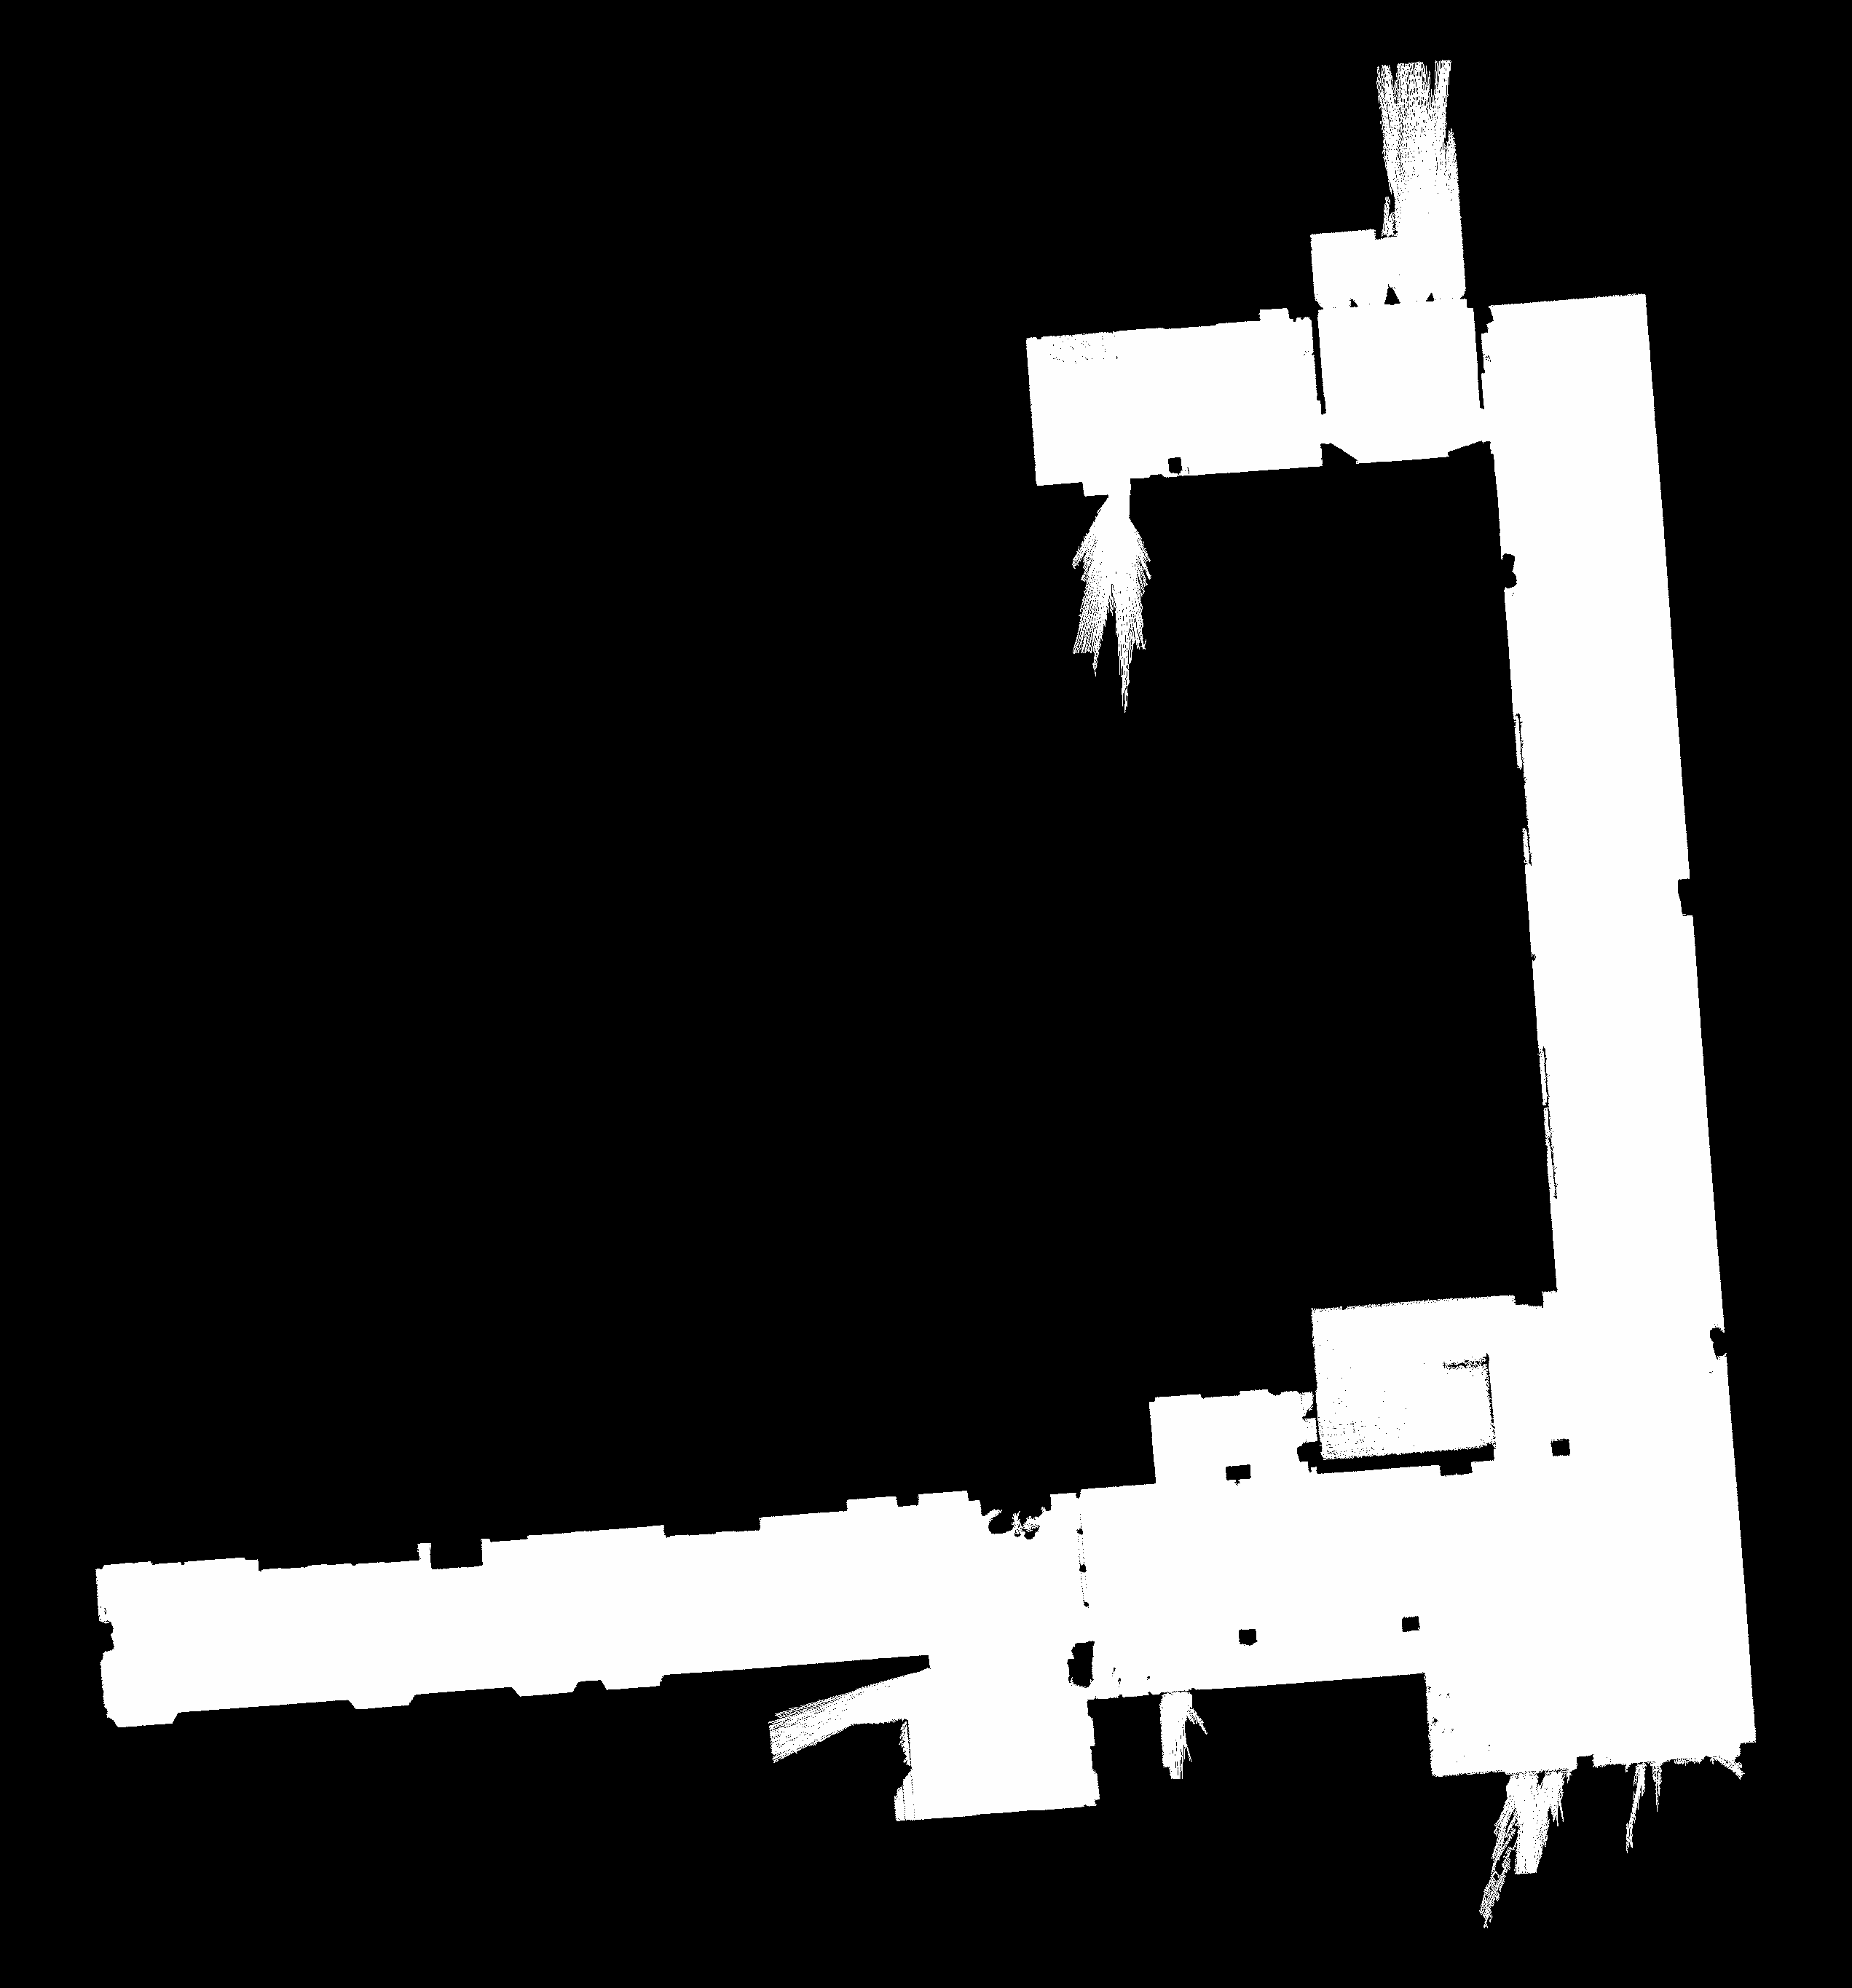
\includegraphics[width=1\textwidth]{figures/franco_map.png}
  \caption{Mappa ottenuta tramite Lidar del primo piano dell'edificio Matematica}
  \label{Mappa ottenuta tramite Lidar del primo piano dell'edificio Matematica}
\end{figure}

\subsection{Localizzazione}
Il terzo test è stato uno dei più importanti, questo riguarda la localizzazione.

\noindent Avendo una mappa dell'ambiente grazie ai test precedenti è stato infatti possibile svolgere test volti al calcolo preciso della propria posizione all'interno di un ambiente conosciuto, questi test grazie al nodo ROS \textbf{particle\_filter}, che implementa l'algoritmo di localizzazione già discusso precedentemente.

\noindent I test di localizzazione condotti hanno evidenziato alcune criticità legate alla natura dell'ambiente di prova. In particolare, sono state riscontrate difficoltà nel raggiungimento di una stima accurata della posizione in determinate aree dell'ambiente, caratterizzate da una scarsità di elementi distintivi (featureless). Tale condizione ha limitato la capacità del filtro a particelle di discriminare tra posizioni potenzialmente simili, compromettendo così la precisione della localizzazione.

\noindent Una soluzione a questo problema può essere sicuramente quella di utilizzare un Lidar più avanzato a tre dimensioni, in modo da apprezzare feature dell'ambiente che non sarebbero altrimenti rilevabili in due dimensioni, soluzione che sta venendo sperimentata al momento della stesura della presente tesi.

\subsection{Guida autonoma}
La sperimentazione conclusiva ha avuto come obiettivo la verifica delle prestazioni complessive del sistema di navigazione autonoma. A partire dalla mappa dell'ambiente generata precedentemente e dai parametri di controllo ottimizzati, è stato pianificato un percorso di riferimento. Successivamente, il robot è stato incaricato di seguire il percorso predefinito, utilizzando l'algoritmo di localizzazione per stimare la propria posizione in tempo reale e adattare la traiettoria in base alle informazioni sensoriali acquisite.

\noindent Sebbene i risultati ottenuti siano stati generalmente positivi, si sono manifestati alcuni problemi di deviazione dalla traiettoria pianificata, attribuibili alle incertezze nella stima di posizione, particolarmente evidenti nelle aree dell'ambiente prive di elementi distintivi.
